\subsection*{Documentation pour l'utilisateur}
Les fonctionnalités du réveil étaient principalement dictées dans l'énoncé du projet. Lors de la mise sous tension du système, l'horloge s'initialise à 00h00m00s (comme un réveil traditionnel). Deux boutons sont présents sur la carte : 
\begin{itemize}
\item Le bouton 1 : il s'agit du bouton du dessous. 
\item Le bouton 2 : il s'agit du bouton placé le plus haut sur la carte.
\end{itemize}
Au démarrage, le réveil affiche un état standard. On peut y voir l'heure défiler. L'alarme est désactivée par défaut, l'heure de celle-ci est initialisée à minuit. \\
En appuyant sur le bouton 1 sur cet état standard, on peut activer/désactiver l'alarme. L'affichage se met alors à jour, indique "Alarm ON" suivi de l'heure sur laquelle il est réglé.\\
Pour ouvrir le menu, il suffit d'appuyer sur le bouton 2. Le réveil propose alors un premier choix, celui de régler l'heure courante. Ré-appuyer sur le bouton 2 affiche l'option suivante du menu : régler l'heure de l'alarme. Pour chacune de ces options, une pression sur le bouton 1 permet d'accéder au paramétrage de l'heure que l'on souhaite modifier. Tandis qu'un troisième appuis sur le boutons 2 nous ramène à l'état initial.\\

Pour modifier une heure, -une fois entré dans le menu adéquat- il suffit d'appuyer sur le bouton 1 pour incrémenter l'unité de temps entre crochet (heure ou minute) d'une unité. Pour valider votre réglage, appuyez sur le bouton 2.\\

Lorsque l'alarme sonne, l'utilisateur est prévenu par un message sur l'écran (l'heure actuelle continue de s'afficher sur la ligne inférieur de l'écran) et les LED rouges clignotent pendant 30 secondes, à raison d'une oscillation par seconde. Une pression sur n'importe quel bouton permet d'arr\^{e}ter la sonnerie. Si l'utilisateur ne modifie ni l'heure courante, ni l'heure d'alarme, le réveil est programmé pour sonner une et unique fois par jour. Il vous est donc possible de réactiver l'alarme dans la m\^{e}me minute que celle où le réveil doit sonner sans qu'il ne déclenche à nouveau. \\

\subsection*{Documentation pour l'installateur}
Notre programme principal ce trouve dans le sous-répertoire \textsc{PIC$\_$AlarmClock} de l'archive \textsc{"Colmonts$\_$VanOuytsel.tar.gzip"}. Il Pour réaliser le programme du réveil, nous sommes à nouveau parti des fichiers donnés comme test avec le projet. Le seul fichier modifié est \textsc{test.c}. Le makefile est donc toujours correct pour compiler l'application à porter sur le PIC. L'utilisation de la commande \textsc{make} est suffisante pour créer le fichier à envoyer.

\subsection*{Documentation pour le programmeur}
Notre programme a été réalisé sur une base très simple. En effet, la majorité du travail consistait à comprendre le fonctionnement de base du PIC. Le programme en lui-m\^{e}me était assez simple à réaliser. Nous avons donc basé notre application sur huit états différents, permettant de savoir ce qu'il faut afficher sur l'écran LCD mais également quelles fonctionnalités possèdent les boutons à chaque instant. Voici un diagramme des transitions entre ces différents états :\\
\begin{center}
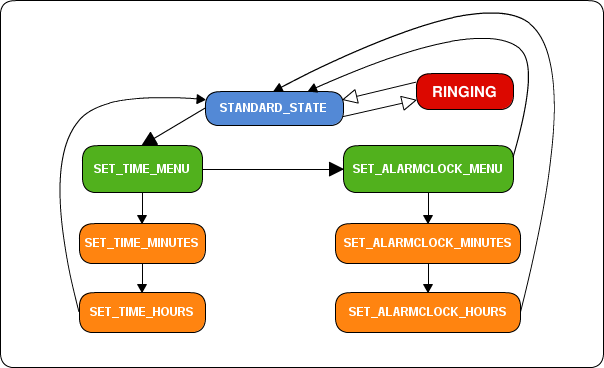
\includegraphics[scale=0.6]{STATE_SCHEMA.png}\\
\end{center}
% DIAGRAMME ETATS
L'élément en bleu est l'état d'affichage standard. Les états en vert sont les états de transition dans le menu principal. Les états en orange concernent les modifications d'heure. Et enfin, l'état en rouge est celui qui s'active lorsque l'alarme $"$sonne$"$.\\
Au niveau des interruptions, il nous semblait évident que le comptage du temps qui passe est bien évidemment l'élément primordial durant toute l'exécution. Les interruptions de haute priorité sont donc utilisée uniquement pour l'overflow du Timer0. Pour avoir le plus de précision possible, nous avons décidé de compter par milliseconde. Le nombre d'incrémentations du Timer0 est d'environ 7000 pour compter cette unité de temps. Comme la taille de celui-ci est de 65536 ($2^{16}$), il n'est pas nécessaire d'utiliser le prescaler.\\
Le second type d'interruptions, celles de basse priorité, sont utilisées pour tout ce qui concerne les boutons. Nous avons considéré qu'il était plus important d'interrompre la routine qui va modifier un état ou l'heure au profit du comptage du temps que de les mettre à un m\^{e}me niveau de priorité.\\
Au niveau de l'affichage LCD, celui-ci se met à jour en permanence dans la boucle du programme principal. Nous évitons ainsi tout affichage dans une interruption (problème de durée de cette opération).